\documentclass[twoside,fontset=fira-newtxsf]{mitthesis}

\usepackage{setspace}
\doublespacing   % common for theses; or \doublespacing

\hypersetup{
  pdfsubject={MIT thesis},
  pdfkeywords={MIT, thesis},
}

\begin{document}

\title{Towards Verifying Correctness and Timing Properties for \\ Out-of-Order Machines}
\Author{Kosi Nwabueze}{Department of Electrical Engineering and Computer Science} [S.B., Massachusetts Institute of Technology (2025)]
\Degree{Master of Engineering}{Department of Electrical Engineering and Computer Science}
\Supervisor{Adam Chlipala}{Professor of Electrical Engineering and Computer Science}
\Acceptor{Katrina LaCurts}{Chair, Master of Engineering Thesis Committee}{}
\DegreeDate{May}{2026}
\ThesisDate{May 8, 2026}

\maketitle

\begin{abstract}
% TODO(kosinw): Write abstract.

\end{abstract}

\chapter*{Acknowledgments}
% TODO(kosinw): Write acknowledgments.

\tableofcontents
\listoffigures
\listoftables

\chapter{Introduction}
This thesis contributes an approach for proving correctness and timing properties for hardware circuits described in the Rocq proof assistant.
This work serves as the first step towards the mechanization of entire correctness and timing proofs for a realistic system including a single out-of-order core and a complete memory hierarchy.

\section{Background: out-of-order execution}
All modern high-speed processors are based on out-of-order (OoO) execution, which allows the CPU to dynamically reorder instructions based on the availability of functional units (FUs) and input operands, minimizing structural hazards.
Instruction scheduling algorithms supporting out-of-order issue and execution started with Tomasulo's algorithm, which first introduced the concept of register renaming to eliminate false dependencies (WAR and RAW hazards) between instructions.
% TODO(kosinw): Add citations for Tomasulo's and register renaming. Add footnotes for RAW and WAR hazards.
Out-of-order execution combined with a separate performance optimizaiton, speculative execution, are vulnerable to transient execution attacks, which in-order processors are not vulnerable to. Principled defenses must be carefully designed to ensure that attackers cannot exploit programs which are safe for in-order processors but unsafe for out-of-order processors.

Figure \ref{fig:fig1} shows a block diagram for the particular variant of the out-of-order algorithm we will consider in this thesis.
We consider a modified design based on the MIPS R10000 (R10K) processor.

\begin{figure}[t!]
  \centering
  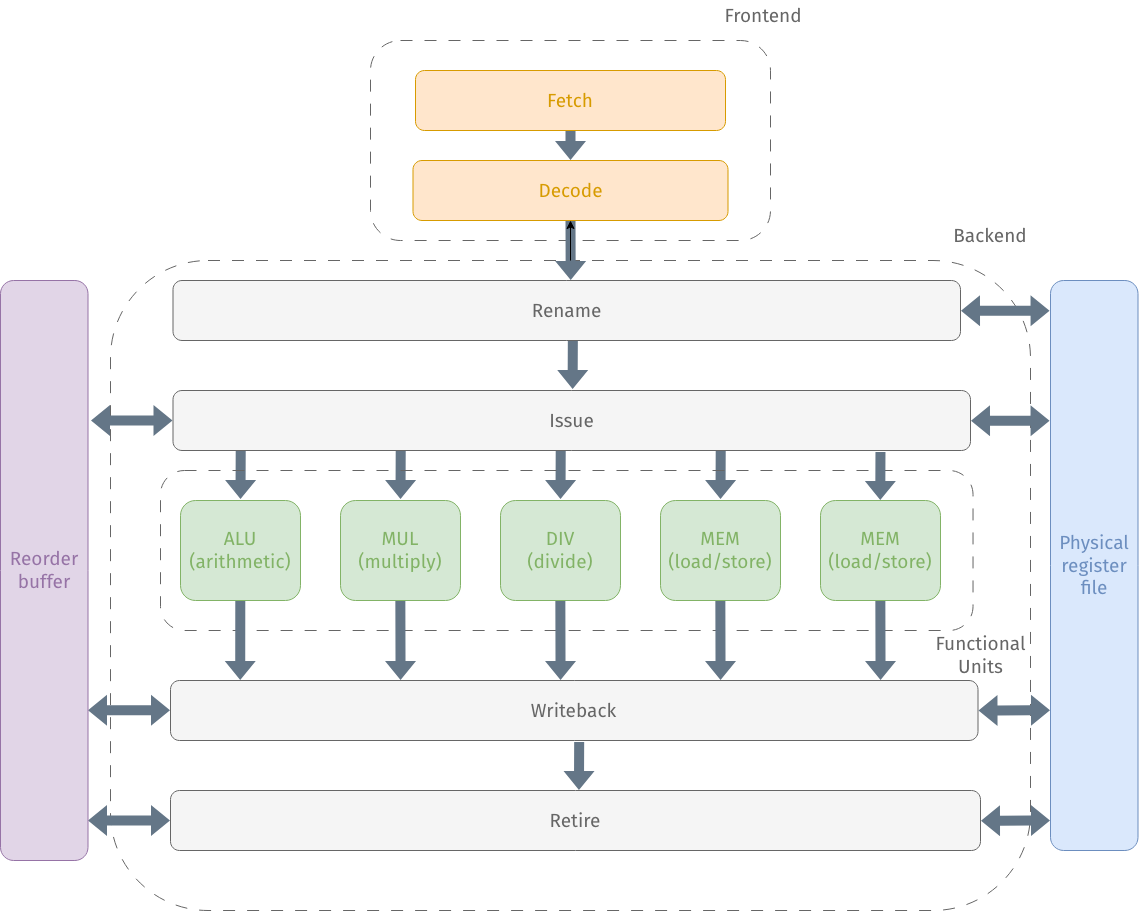
\includegraphics[width=0.75\textwidth]{figures/figure1.png}
  \caption{Diagram for an out-of-order machine based on the R10K processor.}
  \label{fig:fig1}
\end{figure}



Our algorithm is split into seven separate pipeline stages: fetch (F), decode (D), rename (R), issue (I), execute (X), writeback (W), and retire (C).
The front end fetches (F) instructions from the instruction stream and decodes (D) them into an internal data type the machine can schedule.
Rename (R) then maps architectural registers to a larger physical register file so false dependencies (e.g., WAR and WAW hazards) can be dissolved.
Issue (I) selects ready renamed operations and sends them to functional units; which execute the actual computation (e.g., in ALUs or memory units), and writeback (W) posts results to the physical registers so later instructions can consume operands as they become ready.
Retire (C) retires instructions in program order, commiting their effects to the architectural state.
% TODO(kosinw): Add citations for R10K.

Our design diverges from the R10K algorithm in a few important aspects, mostly to simplify which invariants are needed to write proofs.
The most important difference is how the renaming mechanism works
The original R10K algorithm record, in the reorder buffer (ROB), the previous physical register index for each instruction's destination so that the rename map can be rolled back precisely when a younger path is squashed.
We instead avoid tracking that per-instruction previous physical destination in the ROB and instead maintain two register alias tables (RATs).
The \emph{future} table holds the most up-to-date speculative mapping from architectural registers to physical registers, while the \emph{commit} table records the mapping as of the last retired instruction.
Squashing speculative state can then be performed by reverting the \emph{future} back to the \emph{commit} table.

Rolling back the alias tables alone would be insufficient, because speculative execution can still overwrite physical register contents before those instructions retire; restoring only the \emph{architectural-to-physical} (arch-to-phys) mapping would leave stale or partially updated values visible under the recovered names.
Our design therefore pairs the dual RAT with explicit snapshots of register \emph{values} (not just of the rename map).
Enough snapshots are retained to reconstruct the physical register file as it stood at the last retired instruction, so a squash restores both which physical register backs each architectural name and the bit pattern stored in each architectural register at that point.
The maximum number of snapshots is finite, so it bounds the number of branches the machine can speculate ahead; once that budget is exhausted, the issue stage must stall until retire frees snapshot capacity.

A second major deviation concerns speculative memory accesses.
To make timing properties easier to state and prove at first, we delay all speculative loads and stores full stop.
This policy is extremely pessimistic: it sacrifices the performance that comes from speculative execution when interacting with memory, and it is not meant as a proposal for a serious microarchitecture.
Looking ahead, we expect that a more realistic memory design can be recovered by pairing speculative execution with a dynamic taint-tracking defense, together with a mechanized proof that the resulting design still satisfies the same class of timing-security obligations; that extension is left to future work.

\section{Goal: verifying hardware circuits}
This thesis develops techniques for proving correctness and timing properties of synthesizable hardware described in Rocq.
The intended workflow is to state and prove theorems against a source-level circuit semantics, then relate them to synthesizable Verilog through a verified compiler so that the guarantees apply to generated RTL, not only to an informal executable model of the design.

Much related work on mechanized security proofs for hardware reasons about ISA-level models instead of synthesizable circuits.
We focus on synthesizable circuits and verified compilation because that combination pins theorems to descriptions a standard synthesis flow can consume.

\section{Academic context and individual contributions}

\chapter{Related work}

\section{Functional correctness for hardware circuits}
\section{Timing security for hardware circuits}
\section{Verified compilation}

\chapter{Verifying timing properties with state monads}
\section{Specifications}
\section{Implementations}
\section{Proofs}
\section{Discussion}

\chapter{Verifying correctness properties with GoLemma}
\section{Specifications}
\section{Implementations}
\section{Proofs}
\section{Discussion}

\chapter{Case studies}

\section{Timing proof: Multiplier}
\section{Timing proof: Multiple-cycle processor}
\section{Correctness proof: Ring buffer}
\section{Correctness proof: Reorder buffer}

\chapter{Conclusion}
\section{Developer effort}
\section{Discussion}
\section{Future work}

\end{document}
